\chapter{Architecture of the system under test}
\label{chap:architecture}

Due to steady evolvement and increasing requirements the architecture of the system under test has become quite challenging. Physical resources and several software services have been added over the last months. Used software technologies and integration of Tractive's main website and dynamic web application into the whole environment as well as other server components and software tools influence web performance. The following paragraphs give an overview about the infrastructure concerning the web applications and other relevant services.

\section{Infrastructure}
Due to high availability and scalability requirements the main backend services and databases as well as the web application run on dedicated root server instances provided by Hetzner Online GmbH. The hosts are classified into three data-hosts containing our databases (MongoDB, Redis) and three multi-purpose application hosts. Regarding basic performance measurements of the web application the multi-puropse application hosts are relevant. They are optimized for user and hardware traffic and have following technical specifications:

\begin{itemize}
	\item{tractive02 and tractive03}: Intel i7-2600 Quad-Core processor, 32GB DDR3-RAM, 2x 3TB HDD (Software RAID1)
	\item{tractive04}: Intel Core i7-920 Quad- Core processor, 48GB DDR3-RAM, 2x 2TB HDD (Software RAID1)
\end{itemize}

For the backend services as well as the current web application we use the full-stack web framework Ruby on Rails which provides many nice features to build a RESTful web application. Therefore the multi-pupose application host is mainly a Rails Application Server. Besides we have other software components which support us to provide a highly available and scalable web application illustrated in the picture below. 

\begin{figure}[h]
	\centering
		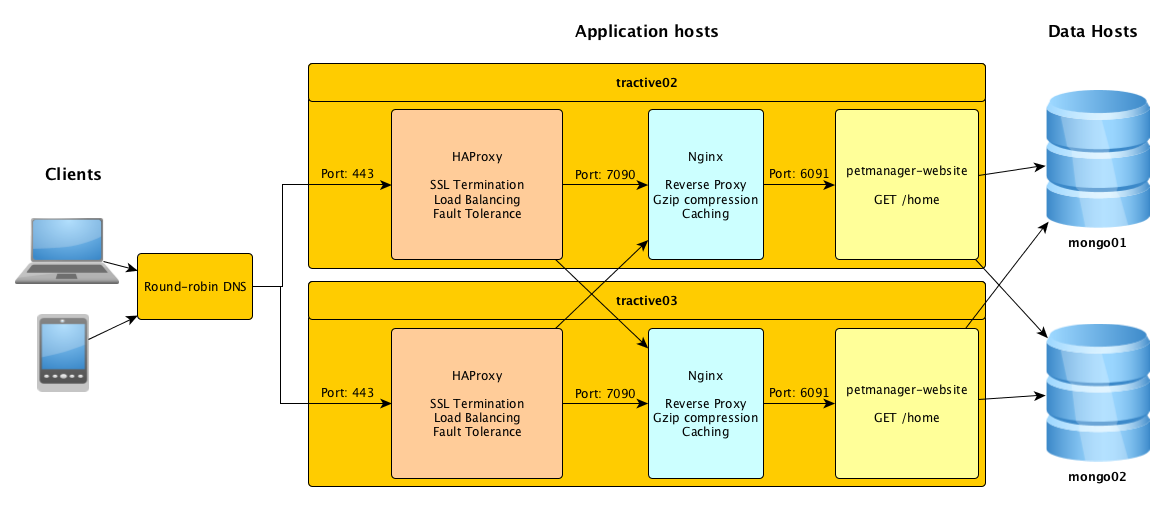
\includegraphics[width=1.0\textwidth]{imgs/architecture.png}
	\caption{Illustration of infrastructure and platform (simplified with only two application and data hosts)}
\end{figure}

Since DNS can hold multiple IP address records for the same domain name it is possible to redirect incoming requests using a Round-robin DNS technique. This algorithm selects the IP addresses of Tractive's three application in an alternating way. A core component of the infrastructure is the HAProxy (High-Availability Proxy) which is the first receiver after an IP-address selection. Incoming requests independent of the type of the service they concern get distributed equally throughout the available servers. In addition to load balancing the HAProxy does health checks and prevents forwarded requests to unavailable services on an instance. Instead such requests are forwarded to a healthy instance. Furthermore HTTPS requests are terminated appropriately and custom ports (protected from outside) are used from this point on. Behind there is a Nginx web server as a powerful component mainly used for caching content, serving assets, providing compression and forwarding requests to the correct service acting as reverse proxy. Especially for static content it allows to return from here directly back when a cache hit was successful. Otherwise the requests gets proxied by and the according service, which for the web application is the petmanager-website service does it's work. In case user-related data is necessary backend algorithms might be triggered and probably the data hosts are required. The petmanager-website collects the necessary information and generates the requested web page dynamically. 
So far a quick overview about the overall infrastructure and it's components before I give some insights into the relevant services. 

\section{Relevant Services}
